\section{Aufbau und Durchführung}
\label{sec:Durchführung}
In diesem Abschnitt werden Aufbau und Durchführung des Experimentes beschrieben.
\subsection{Aufbau}
\label{sec:durchff1}
In Abbildung (\ref{fig:aufbau48}) ist der Aufbau des Versuches und die verwendeten Bauteile zu sehen:
\begin{figure}[h!]
  \centering
  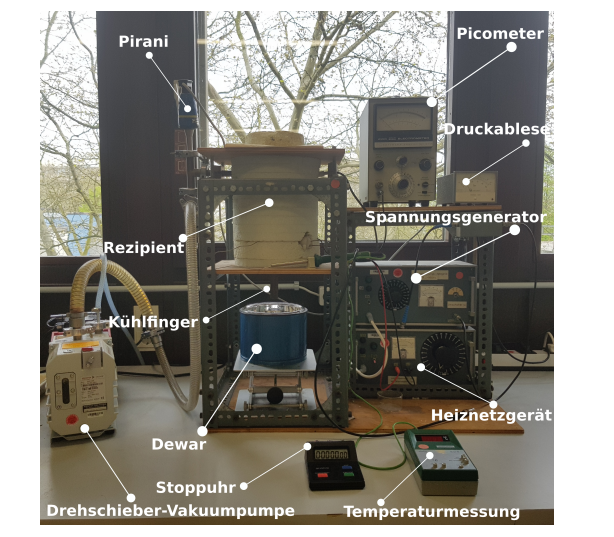
\includegraphics[scale=0.5]{fig/aufbauv48.png}
  \caption{Versuchsaufbau mit beschrifteten Bauteilen \cite[2]{Anleitung1}}
  \label{fig:aufbau48}
\end{figure}
Innerhalb des Rezipienten befindet sich für diesen Versuch als Probe ein Kaliumbromidkristall der mit Strontium dotiert ist. Diese Probe befindet sicht zwischen einer Metallplatte
und dem Boden des Behälters, so entsteht ein Plattenkondensator in dem die Probe als Dielektrikum wirkt. Da der verwendet Kristall hygroskopisch ist wird mithilfe einer Pumpe ein
Vakuum im Rezipienten erzeugt. Dennoch sind einige Wassermoleküle im Rezipienten vorhanden wie später in Abschnitt (\ref{sec:Auswertung}) zu erkennen ist. \\
Im Dewar, der sich unter dem Rezipienten befindet, befindet sich flüssiger Stickstoff, der für die Abkühlung der Probe gebraucht wird. Zum Aufheizen der Probe ist eine Heizspule
im Boden des Behälters verbaut. Gemessen wird die Temperatur der Probe mit einem Thermoelement. in Abbildung (\ref{fig:schema48}) ist dies schematisch dargestellt.
\begin{figure}[h!]
  \centering
  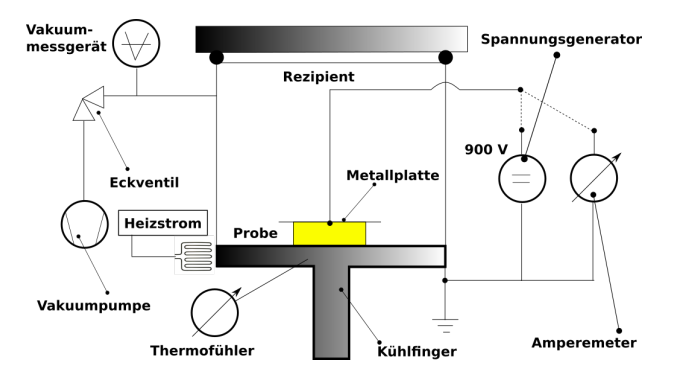
\includegraphics[scale=0.5]{fig/schemav48.png}
  \caption{Schematische Darstellung der Bauteile des Versuches \cite[3]{Anleitung1}}
  \label{fig:schema48}
\end{figure}
\subsection{Durchführung}
\label{sec:durchff2}
Als erstes wird die Probe mithilfe des Plattenkondensators mit einer Spannung von $\SI{950}{\volt}$ etwa 15 Minuten polarisiert, das bedeutet die Dipole werden ausgerichtet. Daraufhin wird die Probe durch den flüssigen Stickstoff im Dewar auf ungefähr $T=\SI{200}{\kelvin}$ abgekühlt und der Kondensator wird zusätzlich einige Minuten kurzgeschlossen, damit die restliche Ladung abfließen kann. \\
Jetzt wird die Probe durch die Heizspule konstant aufgeheizt und die Temperatur um $\Delta T=\SI{100}{\kelvin}$ erhöht, dabei wird pro Minute ein Messwert genommen. Anschließend wird der gesamte Vorgang mit einer
anderen Heizrate wiederholt. Die verwendeten Heizraten sollen für den ersten Durchlauf $\SI{2}{\kelvin\per\minute}$ und für den zweiten Durchlauf $\SI{1.5}{\kelvin\per\minute}$ sein.
